%!TEX root = main.tex
\setcounter{chapter}{2}
\setcounter{section}{3}
\setcounter{theorem}{0}
\setcounter{equation}{0}

\lectureheader{161}{Calculus I}{The definition of limit}{\textit{Thomas' Calculus} \thesection}

\begin{definition}
Let $c\in\R$, and let $f$ be a function so that every open interval containing $c$ also contains points of $\dom(f)$.
We say that the \textbf{limit of $f(x)$ as $x$ approaches $c$ is $L$}, and we write
\begin{equation*}
\lim_{x\to c}f(x) = L,
\end{equation*}
provided that for every $\epsilon>0$, there is a $\delta>0$ so that 
\begin{equation*}
x\in\dom(f)\text{ and }0<|x-c|<\delta \implies |f(x) - L|<\epsilon.
\end{equation*}
\end{definition}

\begin{remark}\,
\begin{itemize}
\item
If the limit exists, then given any $\epsilon>0$, we can find a $\delta>0$ so that if we make sure $x$ is within $\delta$ of $c$, then $y=f(x)$ will be within $\epsilon$ of $L$.
\item 
The Greek letter $\epsilon$ is meant to remind us of the word ``error."  It is the allowable ``error tolerance" in the output.
\item
Our job is to control this output error through the input variable by finding the appropriate tolerance $\delta$ on the input.
\end{itemize}
\end{remark}

\begin{example}
Our intuition already tells us that $\DS\lim_{x\to 3}f(x) = 5$ if 
\begin{equation*}
f(x) = \begin{cases} 2x-1, & x\ne 3\\ 6, & x=3.\end{cases}
\end{equation*}
How close (but not equal) to $3$ does $x$ have to be to ensure that $f(x)$ is within $\epsilon = 0.1$ of $L=5$?
\end{example}
\begin{flushright}
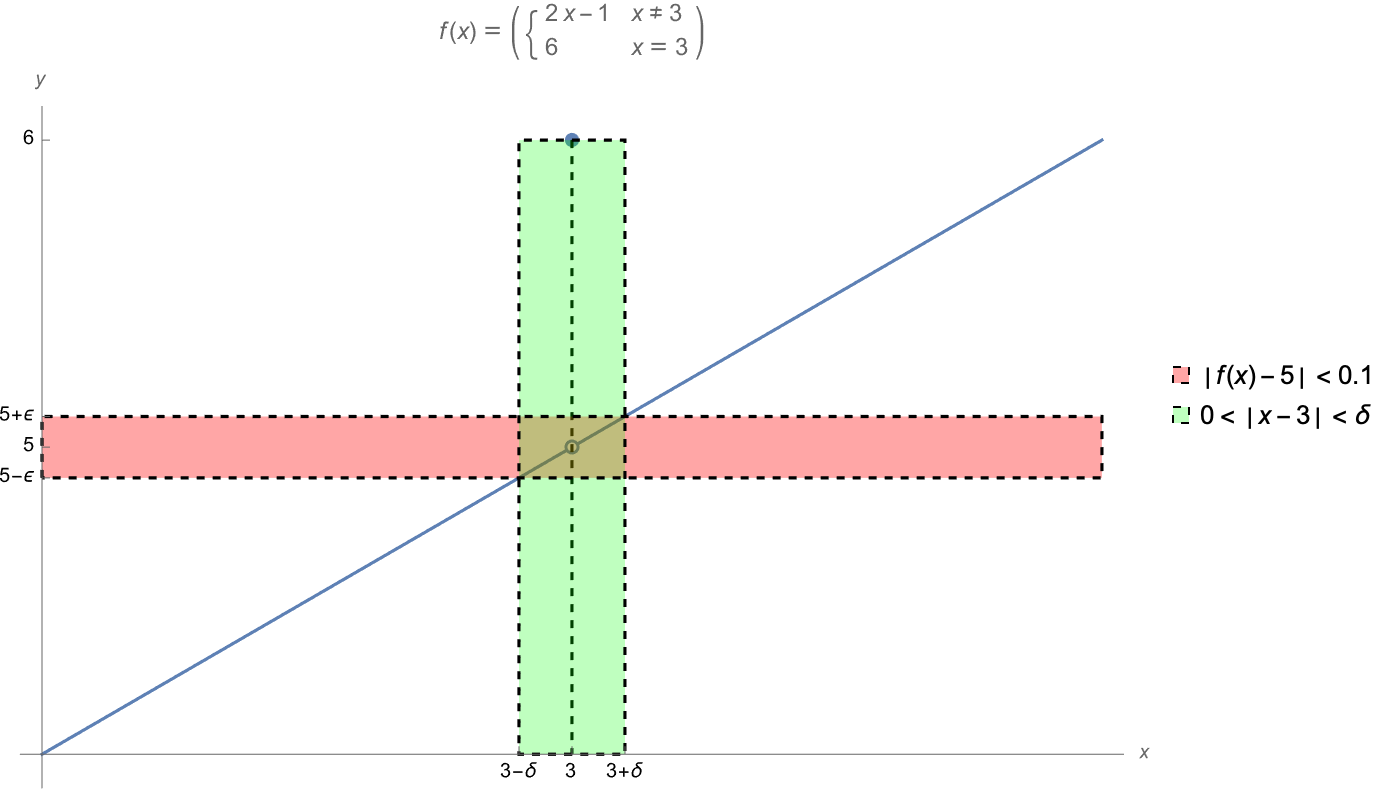
\includegraphics[width=3.5in]{img/epsilon-delta-ex1}
\end{flushright}

\newpage

\begin{example}
Prove that $\DS\lim_{x\to 3}(4x-5)=7$.
\end{example}

\newpage

\begin{example}
Prove that $\DS\lim_{x\to 2}x^2=4$.
\end{example}

\newpage

\begin{example}
Prove that $\DS\lim_{x\to 5}\sqrt{x-1} = 2$.
\end{example}

\newpage

\begin{example}
If $\DS\lim_{x\to c}f(x) = L$ and $\DS\lim_{x\to c}g(x) = M$, prove that $\DS\lim_{x\to c}\big(f(x)+g(x)\big) = L+ M$.
\end{example}

